\documentclass[12pt,a4paper]{report}

% ==================== PACKAGES ====================
\usepackage[a4paper,margin=1in]{geometry}
\usepackage{graphicx}
\usepackage{xcolor}
\usepackage{setspace}
\usepackage{fancyhdr}
\usepackage{titlesec}
\usepackage{hyperref}
\usepackage{float}
\usepackage{caption}
\usepackage{enumitem}
\usepackage{amsmath,amssymb}
\usepackage{booktabs}
\usepackage{tabularx}

% ==================== FORMATTING & STYLING ====================
\onehalfspacing
\setlength{\parindent}{0pt}
\setlength{\parskip}{6pt}

\hypersetup{
    colorlinks=true,
    linkcolor=black,
    urlcolor=blue,
    citecolor=blue,
    pdftitle={AI Network Infrastructure: End-to-End Inference Architecture},
    pdfauthor={Karan Bhojak}
}

% Chapter and Section Headings
\titleformat{\chapter}[display]
{\normalfont\huge\bfseries}{\chaptertitlename\ \thechapter}{10pt}{\Huge}
\titlespacing*{\chapter}{0pt}{-20pt}{20pt}

\titleformat{\section}
{\normalfont\Large\bfseries}{\thesection}{1em}{}

\titleformat{\subsection}
{\normalfont\large\bfseries}{\thesubsection}{1em}{}

% Header and Footer
\pagestyle{fancy}
\fancyhf{}
\fancyhead[L]{AI Network Infrastructure}
\fancyhead[R]{Karan Bhojak}
\fancyfoot[C]{\thepage}
\renewcommand{\headrulewidth}{0.4pt}

% ==================== DOCUMENT ====================
\begin{document}

% ==================== COVER PAGE ====================
\begin{titlepage}
    \centering

    \vspace*{1.5cm}

    {\Huge\bfseries AI Network Infrastructure\par}
    \vspace{0.4cm}
    {\LARGE\bfseries High-Level End-to-End Network Infrastructure for AI Inference Systems\par}
    \vspace{0.3cm}
    {\large\textit{A Detailed Technical Examination of the Prompt Request Lifecycle from Client to GPU and Back}\par}

    \vspace{1.5cm}

    {\Large Academic Report\par}

    \vspace{2cm}

    {\large Submitted By:\par}
    \vspace{0.3cm}
    {\Large\bfseries KARAN BHOJAK\par}

    \vspace{1.5cm}

    {\large Submitted To:\par}
    {\large [Faculty Name]\par}

    \vspace{1cm}

    {\large [College Name]\par}

    \vfill

    {\large Academic Year: 2026--2027\par}

    \vspace{1cm}
\end{titlepage}

% ==================== PRELIMINARY PAGES ====================
\pagenumbering{roman}

% Abstract
\chapter*{Abstract}
\addcontentsline{toc}{chapter}{Abstract}

Artificial Intelligence (AI) and Large Language Models (LLMs) have evolved into foundational technologies powering intelligent conversational agents, real-time code completion tools, and automated enterprise workflows. These interactive applications depend upon a specialized, high-performance network infrastructure capable of receiving user prompts, securely transporting data across global networks, distributing computational loads across enterprise data center fabrics, and returning generated text with minimal latency.

In traditional web applications, network communication follows a predictable request-response model where static files or pre-computed database records are retrieved and returned in a single transmission. Conversely, AI inference systems introduce unique computational requirements: input prompts must be tokenized, batched dynamically, and processed across distributed clusters of Graphics Processing Units (GPUs) performing billions of simultaneous floating-point operations. Furthermore, because language models generate text autoregressively (one token at a time), network architectures must support persistent, low-latency streaming channels that deliver tokens back to the user incrementally.

This report provides a comprehensive, structured analysis of the end-to-end network infrastructure that supports modern AI inference systems. Following the path of a user prompt, the report examines each architectural layer in detail: starting from client endpoints (smartphones and laptops), moving through public Internet routing, traversing Content Delivery Network (CDN) edge locations, entering regional data centers via redundant border routers, navigating non-blocking spine-leaf switching fabrics, undergoing Layer 7 load balancing and API gateway inspection, being scheduled across inference worker pools, and executing across interconnected GPU accelerators.

By explaining complex networking and distributed computing concepts through clear, accessible computer science principles, this report serves as an accessible yet technically rigorous guide to the hardware, protocols, and operational workflows that enable modern artificial intelligence.

\clearpage

% Table of Contents
\tableofcontents
\addcontentsline{toc}{chapter}{Contents}

\clearpage
\listoffigures
\addcontentsline{toc}{chapter}{List of Figures}

\clearpage

% ==================== CHAPTER 1 ====================
\pagenumbering{arabic}

\chapter{Introduction and Architectural Overview}

\section{Background: The Operational Requirements of Modern AI}
In contemporary computing, user interaction with Artificial Intelligence (AI) models—such as Large Language Models (LLMs)—presents distinct challenges that differ fundamentally from standard Internet services. When an individual submits a text query (commonly referred to as a \textit{prompt}) to an AI platform, the system does not simply retrieve a stored document from a database. Instead, it must dynamically evaluate the prompt using a neural network consisting of tens or hundreds of billions of numerical parameters and generate a contextually relevant response.

This operational paradigm introduces several critical performance constraints:
\begin{enumerate}[leftmargin=1.2cm]
    \item \textbf{Low Latency Expectation:} Users interact with AI systems conversationally. Any noticeable delay between submitting a query and observing the initial response degrades the user experience.
    \item \textbf{Autoregressive Generation:} Large Language Models generate text sequentially. Each output word (or token) is produced by evaluating the initial prompt combined with all preceding generated words. As a result, the network cannot wait for the entire answer to be compiled before transmitting data; it must stream output incrementally in real time.
    \item \textbf{Statefulness and Memory Footprint:} Unlike stateless web services where any server can process any incoming request independently, LLM inference requires maintaining continuous memory states (such as attention Key-Value caches) across the duration of the generation session.
\end{enumerate}

Meeting these requirements requires an infrastructure engineered specifically for high bandwidth, deterministic routing, and minimal communication jitter.

\section{Traditional Web Architecture vs. AI Inference Infrastructure}
To understand the necessity of specialized AI networks, it is useful to compare AI inference with traditional web architectures (often categorized as Web 2.0).

In a traditional web application (such as an online retail store or an encyclopedia):
\begin{itemize}[leftmargin=1.2cm]
    \item A client sends a standard HTTP \texttt{GET} or \texttt{POST} request.
    \item A web server receives the request, queries a relational database, and retrieves stored data.
    \item The server compiles the response into a complete HTML page or JSON object and transmits it back to the client as an atomic, single payload.
    \item Network load is primarily \textbf{North--South} (between client and server), with low inter-server communication requirements.
\end{itemize}

In an AI inference application:
\begin{itemize}[leftmargin=1.2cm]
    \item The prompt is ingested and converted into mathematical vectors (tensors).
    \item The workload is heavily computational: billions of matrix multiplication calculations must be completed within milliseconds.
    \item Because state-of-the-art models exceed the memory capacity of an individual processor, model weights are distributed across multiple GPUs. This creates massive internal data exchange requirements between computing nodes.
    \item The response is delivered as a continuous stream of data packets over an extended, open connection.
\end{itemize}

Table~\ref{tab:comparison_web_ai} summarizes these operational differences.

\begin{table}[H]
\centering
\caption{Technical Comparison: Traditional Web Applications vs. AI Inference Systems}
\label{tab:comparison_web_ai}
\begin{tabularx}{\textwidth}{lXX}
\toprule
\textbf{Attribute} & \textbf{Traditional Web Applications} & \textbf{AI Inference Systems} \\
\midrule
\textbf{Workload Characteristics} & I/O bound (database reads, file access) & Compute and memory-bandwidth bound \\
\textbf{Response Delivery} & Single atomic payload (HTTP 200 OK) & Incremental token streaming (Server-Sent Events) \\
\textbf{Compute Node Types} & General-purpose Central Processing Units (CPUs) & Specialized Graphics Processing Units (GPUs) \\
\textbf{Internal Network Traffic} & Moderate inter-server queries & Massive, microsecond-latency tensor transfers \\
\textbf{Session State} & Stateless application servers; shared cache & Stateful Key-Value cache pinned to GPU memory \\
\textbf{Packet Delay Tolerance} & High tolerance (TCP retransmission suffices) & Extremely low tolerance (tail latency stalls GPUs) \\
\bottomrule
\end{tabularx}
\end{table}

\section{Traffic Classification: North--South Ingress vs. East--West Interconnects}
In enterprise networking, data flows are categorized based on their directional traversal:
\begin{itemize}[leftmargin=1.2cm]
    \item \textbf{North--South Traffic:} Refers to network packets traveling between external clients (smartphones, personal computers) and the data center. This pathway focuses on wide-area reachability, protocol negotiation, transport-layer encryption, security filtering, and client connection management.
    \item \textbf{East--West Traffic:} Refers to network packets moving entirely within the boundaries of the data center, specifically between servers, storage clusters, and individual GPU compute nodes. In an AI environment, East--West traffic demands non-blocking, multi-terabit bandwidth and microsecond-level latency to support distributed tensor operations.
\end{itemize}

\section{The System Architectural Blueprint}
Figure~\ref{fig:ai_architecture} illustrates the reference architecture of a modern end-to-end AI inference system. This diagram serves as the structural foundation for the remainder of this report.

\begin{figure}[H]
    \centering
    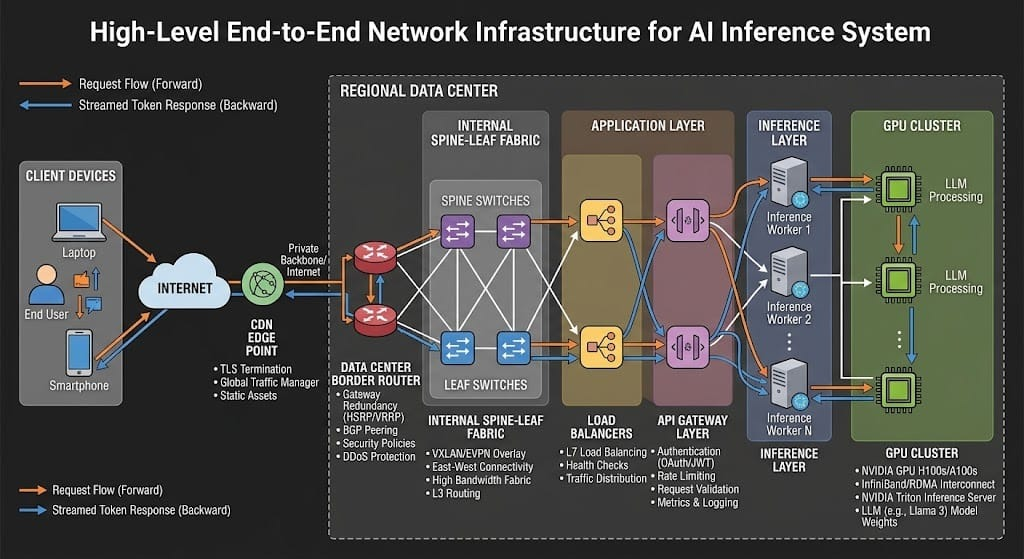
\includegraphics[width=\textwidth]{ai_architecture.jpg}
    \caption{High-Level End-to-End Network Infrastructure for AI Inference System}
    \label{fig:ai_architecture}
\end{figure}

As depicted in Figure~\ref{fig:ai_architecture}, the end-to-end system comprises several distinct architectural zones:
\begin{enumerate}[leftmargin=1.2cm]
    \item \textbf{Client Devices:} External endpoints where prompts originate and streamed responses are displayed.
    \item \textbf{Internet and CDN Edge Point:} The global public transport layer and local edge caching/security infrastructure.
    \item \textbf{Regional Data Center Perimeter:} The entrance boundary managed by redundant Data Center Border Routers.
    \item \textbf{Internal Spine-Leaf Fabric:} The high-speed switching fabric providing uniform Layer 3 transport within the facility.
    \item \textbf{Application Layer:} The ingestion and governance tier consisting of Layer 7 Load Balancers and API Gateways.
    \item \textbf{Inference Layer:} Orchestration nodes (Inference Workers) responsible for queueing, tokenization, and dynamic batching.
    \item \textbf{GPU Cluster:} High-performance compute clusters executing the neural network calculations over low-latency fabrics.
\end{enumerate}

Throughout this system, two continuous data streams operate simultaneously:
\begin{itemize}
    \item \textbf{Forward Request Flow (Orange Arrows):} The forward journey of the prompt from the user device into the GPU cluster.
    \item \textbf{Streamed Token Response (Blue Arrows):} The reverse journey of generated tokens streaming back to the user.
\end{itemize}

% ==================== CHAPTER 2 ====================
\chapter{The Ingress Journey: From User Device to the CDN Edge}

In this chapter, we trace the initial leg of the prompt's journey: originating at the user's computing device, traversing the public Internet, and terminating at the Content Delivery Network (CDN) edge facility.

\section{The Client Device Tier: Prompt Generation and Transmission}
The lifecycle of an AI prompt begins when an end user enters text into an application running on a personal computer (laptop or desktop) or a mobile device (smartphone or tablet), as shown on the far left of Figure~\ref{fig:ai_architecture}.

\subsection{Prompt Construction and Payload Encapsulation}
When the user submits a prompt, the client application (such as a web application running in a browser or a native mobile application) encapsulates the text into a structured application-layer packet, typically formatted as a JSON (JavaScript Object Notation) payload. 

A representative prompt payload contains the following standardized fields:
\begin{itemize}[leftmargin=1.2cm]
    \item \textbf{Model Identifier:} Specifies the targeted neural network (for example, \texttt{"model": "llama-3-70b-instruct"}).
    \item \textbf{Message History:} Contains the user's current prompt along with optional preceding conversational context to allow conversational continuity.
    \item \textbf{Generation Parameters:} Defines execution settings such as temperature (sampling diversity) and maximum token limits.
    \item \textbf{The Streaming Directive:} A dedicated boolean flag (\texttt{"stream": true}). This parameter explicitly instructs downstream servers not to hold the completed answer, but rather to establish a persistent streaming pipeline back to the client.
\end{itemize}

\subsection{Local Network Egress}
Once encapsulated, the client operating system passes the data to its transport layer stack. The payload is divided into TCP segments (or UDP datagrams if utilizing modern HTTP/3 over QUIC protocols). 

The device's physical network adapter—either a Wi-Fi interface (IEEE 802.11) or a cellular radio interface (5G/4G-LTE)—modulates the digital bits into high-frequency electromagnetic signals, transmitting them to the local wireless access point or cellular base station.

\section{Public Internet Routing: Transport Across Global Networks}
After departing the local network, the user's data packets enter the public Internet (represented by the Internet cloud in Figure~\ref{fig:ai_architecture}).

\subsection{Domain Name Resolution and Anycast Routing}
To direct packets to the service, the client device first resolves the human-readable domain name (such as \texttt{api.provider.ai}) into a numerical Internet Protocol (IP) address via the Domain Name System (DNS).

Leading AI infrastructure providers employ **BGP Anycast** addressing. In standard unicast routing, an IP address belongs to a single physical machine in one location. Under Anycast, the identical IP address is advertised simultaneously by hundreds of data centers and edge facilities globally. 

Through standard Internet routing protocols, the client's local Internet Service Provider (ISP) automatically forwards the prompt packets to the topologically closest edge facility, significantly reducing the initial network round-trip time.

\subsection{Internet Latency and Jitter}
The public Internet is an unmanaged, shared network composed of multiple independent Autonomous Systems (AS). Packets may experience variable delays (jitter) and routing fluctuations. If client requests were required to travel directly from user devices across the public Internet to a distant central data center, the connection setup phase would suffer substantial latency penalties. To solve this, the request is intercepted at the network edge by a Content Delivery Network.

\section{The Content Delivery Network (CDN) Edge Point}
The **CDN Edge Point** (or Point of Presence / PoP) represents a distributed edge facility deployed near local Internet Exchange Points (IXPs) and telecommunication hubs. As highlighted in Figure~\ref{fig:ai_architecture}, the CDN Edge Point executes three primary functions:

\subsection{1. TLS Termination}
Modern web communications mandate end-to-end encryption using Transport Layer Security (TLS 1.3). Setting up a secure TLS session requires a multi-step cryptographic handshake between client and server, exchanging digital certificates and calculating symmetric encryption keys.
\begin{itemize}[leftmargin=1.2cm]
    \item \textbf{Operational Workflow:} The CDN Edge Point performs **TLS Termination**. It completes the cryptographic handshake with the user's device locally, typically within 5 to 15 milliseconds.
    \item \textbf{Engineering Advantage:} By terminating TLS at the edge, the computationally intensive cryptographic negotiation is resolved near the user. The decrypted prompt payload can then be accelerated across optimized infrastructure, eliminating intercontinental handshake round-trips.
\end{itemize}

\subsection{2. Global Traffic Management (GTM)}
A global AI platform operates multiple regional data centers worldwide. Because AI workloads consume vast computational resources, individual data centers may periodically experience capacity saturation or localized infrastructure faults.
\begin{itemize}[leftmargin=1.2cm]
    \item \textbf{Operational Workflow:} The CDN functions as an active **Global Traffic Manager**. It continuously evaluates health metrics, available GPU queue capacity, and network latency reports across all downstream regional data centers.
    \item \textbf{Intelligent Routing:} If a primary data center is under heavy load or offline for maintenance, the GTM automatically directs incoming prompt streams to the nearest operational data center possessing available compute capacity.
\end{itemize}

\subsection{3. Static Asset Caching}
An AI application interface requires various static resources to function, including JavaScript bundles, user interface stylesheets (CSS), image icons, and font files.
\begin{itemize}[leftmargin=1.2cm]
    \item \textbf{Operational Workflow:} The CDN caches these unchanging assets in local solid-state storage at the edge.
    \item \textbf{Resource Optimization:} When a user loads the AI web portal, all static visual elements are served directly from the local CDN edge. This prevents non-computational traffic from traversing data center networks, reserving data center bandwidth strictly for dynamic inference queries.
\end{itemize}

\section{Dedicated Backbone Transit: Transitioning to the Private Network}
Once the prompt payload has been received and inspected at the CDN Edge Point, it departs the public Internet. 

To guarantee low latency and consistent throughput, hyperscale AI operators route the prompt across a **Private Backbone** (labeled in Figure~\ref{fig:ai_architecture} between the CDN and the Regional Data Center). This private network consists of leased or dedicated high-capacity optical fiber lines. By avoiding public Internet transit, the request travels to the destination regional data center under deterministic Quality of Service (QoS) guarantees, completely shielded from external congestion.

% ==================== CHAPTER 3 ====================
\chapter{Regional Data Center Entry: The Border Router and Perimeter Defense}

In this chapter, the prompt reaches the boundary of the **Regional Data Center** (represented by the large dashed container in Figure~\ref{fig:ai_architecture}). Here, we examine the network components responsible for facility ingress, routing coordination, and perimeter security.

\section{The Data Center Border Router: The Network Perimeter}
The entry point into the physical data center is the **Data Center Border Router**. Border routers are high-capacity, carrier-grade routing systems equipped with multi-terabit switching fabrics. They serve as the demarcation boundary between external networks (the private backbone and upstream transit carriers) and the internal data center switching fabric.

As detailed in the architecture diagram, the border router operates four mission-critical capabilities: gateway redundancy, routing protocol peering, security policy enforcement, and anti-DDoS scrubbing.

\section{Gateway Redundancy (HSRP / VRRP): Ensuring High Availability}
In an enterprise environment serving millions of continuous concurrent connections, the failure of a primary ingress router would disconnect active sessions and render the data center unreachable.

To eliminate single points of failure, border routers are deployed in redundant, dual-homed pairs utilizing standardized gateway redundancy protocols:
\begin{itemize}[leftmargin=1.2cm]
    \item \textbf{VRRP (Virtual Router Redundancy Protocol - RFC 5798):} An open-standard protocol in which two physical routers share a common Virtual IP (VIP) address. One physical router is designated as the active master, while the second remains in a hot-standby state.
    \item \textbf{HSRP (Hot Standby Router Protocol):} A comparable high-availability protocol commonly implemented in Cisco networking environments.
    \item \textbf{Operational Mechanism:} The two routers continuously exchange sub-second heartbeat messages (keepalives). If the active router experiences a power failure, interface failure, or software crash, the standby router detects the loss within milliseconds and assumes forwarding responsibility for the Virtual IP address without disrupting established client connections.
\end{itemize}

\section{BGP Peering: Autonomous System Path Optimization}
To coordinate routing with external networks, data center border routers run **BGP (Border Gateway Protocol)**, specifically external BGP (eBGP).

\begin{itemize}[leftmargin=1.2cm]
    \item \textbf{Route Advertisement:} The border routers maintain continuous peering sessions with upstream Internet Service Providers and private backbone routers, advertising the data center's assigned IP prefixes.
    \item \textbf{Path Selection:} BGP evaluates autonomous system paths, Multi-Exit Discriminators (MED), and local preference metrics to select the most efficient physical path for incoming traffic, ensuring that prompt packets enter the data center through optimal fiber circuits.
\end{itemize}

\section{Perimeter Security Policies and Access Control}
AI compute clusters represent significant capital investments and are frequent targets for unauthorized access and cyber reconnaissance. The border router acts as an initial security perimeter by enforcing hardware-level **Security Policies**:
\begin{itemize}[leftmargin=1.2cm]
    \item \textbf{Access Control Lists (ACLs):} Stateless packet filters implemented in specialized switch hardware (Ternary Content-Addressable Memory, or TCAM). These filters inspect IP packet headers at line rate, immediately dropping unauthorized protocols, spoofed IP addresses, and traffic targeting closed internal subnets.
    \item \textbf{Stateful Inspection:} Verifies that incoming packets correspond to legitimate, actively negotiated transport sessions.
\end{itemize}

\section{Distributed Denial of Service (DDoS) Mitigation}
A primary operational hazard for public-facing AI endpoints is a Distributed Denial of Service (DDoS) attack, where coordinated botnets flood an infrastructure with malicious traffic to exhaust compute or network resources.

\begin{itemize}[leftmargin=1.2cm]
    \item \textbf{Inline Traffic Scrubbing:} Dedicated DDoS mitigation hardware is integrated directly into the border routing layer.
    \item \textbf{Anomaly Detection:} The scrubbing system monitors incoming flow telemetry (such as NetFlow or sFlow metrics). When abnormal traffic volumes (e.g., SYN floods or UDP reflection bursts) are detected, the system diverts the traffic through hardware scrubbing centers.
    \item \textbf{Sanitization:} Malicious volumetric packets are filtered and discarded, while legitimate user prompt traffic is permitted through to the internal network unimpeded.
\end{itemize}

Having passed through perimeter verification, the prompt packet is routed into the internal switching fabric of the data center.

% ==================== CHAPTER 4 ====================
\chapter{Inside the Regional Data Center: Compute and Fabric Infrastructure}

Chapter 4 examines the physical and logical interior of the data center. This constitutes the largest and most critical section of the report, encompassing the internal network fabric, the application ingestion layer, the inference orchestration layer, and the GPU cluster.

\section{The Internal Spine-Leaf Switching Fabric}
Once past the border router, the prompt packet enters the data center's local area network. In an AI infrastructure, traditional hierarchical enterprise network designs are incapable of meeting performance requirements.

\subsection{Why Traditional Hierarchical Networks Are Replaced}
Historically, data centers utilized a three-tier network hierarchy: Core, Distribution, and Access layers, linked together using the Spanning Tree Protocol (STP). 
\begin{itemize}[leftmargin=1.2cm]
    \item \textbf{The Bottleneck:} In STP-based topologies, redundant network links must be logically disabled to prevent packet loops. This wastes up to 50\% of installed network cabling.
    \item \textbf{Variable Latency:} Communication latency between servers varies widely depending on how many switch tiers a packet must traverse, creating severe performance degradation for distributed computing tasks.
\end{itemize}

Modern AI facilities replace this model with an **Internal Spine-Leaf Fabric** (derived from the multi-stage Clos network topology), as illustrated in the center of Figure~\ref{fig:ai_architecture}.

\subsection{Spine Switches and Leaf Switches}
The Spine-Leaf architecture organizes network switches into two functional layers:
\begin{enumerate}[leftmargin=1.2cm]
    \item \textbf{Leaf Switches (Top-of-Rack / ToR):} Represented by the lower blue switch tier in Figure~\ref{fig:ai_architecture}. A pair of redundant Leaf switches is installed at the top of every physical server rack. All servers, load balancers, and compute nodes within that rack connect directly to these Leaf switches.
    \item \textbf{Spine Switches:} Represented by the upper purple switch tier in Figure~\ref{fig:ai_architecture}. Spine switches form the high-speed distribution backbone of the data center.
\end{enumerate}

\subsection{The Two-Hop Latency Guarantee}
The fundamental design rule of a Spine-Leaf fabric is strictly enforced:
\begin{center}
    \textit{Every Leaf switch is connected to every Spine switch, while Leaf switches never connect to other Leaf switches, and Spine switches never connect to other Spine switches.}
\end{center}

This structure guarantees that any server in the facility can communicate with any other server across **exactly two switch hops**:
\begin{equation}
    \text{Source Server} \longrightarrow \text{Ingress Leaf} \longrightarrow \text{Spine Switch} \longrightarrow \text{Egress Leaf} \longrightarrow \text{Destination Server}
\end{equation}
This delivers uniform, predictable, and non-blocking microsecond latency across the entire facility.

\subsection{High Bandwidth Fabric and East--West Connectivity}
The inter-switch connections within the spine-leaf fabric utilize high-density optical transceivers providing **400 Gbps to 800 Gbps** per link. This massive bandwidth capacity provides non-blocking East--West communication, ensuring that internal microservices and computing racks exchange data without encountering network contention.

\subsection{Layer 3 ECMP (Equal-Cost Multi-Path) Routing}
Routing within the fabric operates at Layer 3 (IP routing) rather than Layer 2 (Ethernet switching), completely eliminating Spanning Tree Protocol limitations.
\begin{itemize}[leftmargin=1.2cm]
    \item \textbf{Operational Workflow:} When a Leaf switch forwards a packet toward a destination, it identifies multiple parallel Spine switches offering identical path costs.
    \item \textbf{ECMP Hashing:} The Leaf switch computes a mathematical hash of the packet's 5-tuple header (Source IP, Destination IP, Source Port, Destination Port, and Protocol). Based on this hash, the flow is assigned to one of the parallel uplinks.
    \item \textbf{Result:} Traffic is distributed evenly across all available Spine switches, maximizing aggregate throughput and providing seamless failover if an individual switch link fails.
\end{itemize}

\subsection{VXLAN and BGP EVPN Network Virtualization}
To maintain security isolation between different operational environments without physical recabling, modern data centers implement network overlay virtualization:
\begin{itemize}[leftmargin=1.2cm]
    \item \textbf{VXLAN (Virtual Extensible LAN - RFC 7348):} Encapsulates Layer 2 Ethernet frames inside standard Layer 3 UDP datagrams. This allows logical subnets to extend seamlessly across the routed spine-leaf physical network (underlay).
    \item \textbf{BGP EVPN (Ethernet VPN - RFC 8365):} Acts as the control plane protocol for VXLAN, automatically synchronizing host reachability and MAC address tables across all Leaf switches, eliminating unnecessary broadcast traffic.
\end{itemize}

Through this fabric, the user's prompt is delivered to the rack hosting the **Application Layer**.

\section{The Application Layer: Ingestion and Governance}
The Application Layer serves as the gateway for request ingestion, traffic normalization, and security compliance before any query reaches specialized AI compute hardware. It consists of two sub-layers: **Load Balancers** and **API Gateways**.

\subsection{Layer 7 Load Balancers}
As shown in Figure~\ref{fig:ai_architecture}, incoming requests first reach the **Load Balancers** (implemented using advanced reverse-proxy software such as Envoy Proxy or HAProxy).

The load balancer performs three critical tasks:
\begin{enumerate}[leftmargin=1.2cm]
    \item \textbf{Layer 7 Protocol Parsing:} Unlike basic Layer 4 load balancers that inspect only IP addresses and TCP ports, a Layer 7 proxy inspects the actual application layer content. It terminates incoming HTTP/2 or HTTP/3 sessions, decodes request headers, and manages multiplexed gRPC connections.
    \item \textbf{Active Health Checks:} The load balancer continuously executes synthetic health checks against downstream API Gateway and worker instances. If a target node displays elevated response latencies, memory exhaustion, or error codes, the load balancer dynamically removes it from the routing pool.
    \item \textbf{Intelligent Traffic Distribution:} Instead of basic round-robin distribution, the load balancer utilizes algorithms such as \textit{Weighted Least Request} or \textit{Peak Exponentially Weighted Moving Average (PEWMA)}. Requests are dynamically routed to the specific server possessing the lowest active queue depth.
\end{enumerate}

\subsection{The API Gateway Layer}
Directly downstream of the load balancers sits the **API Gateway Layer**. The API Gateway serves as the centralized enforcement point for operational policies, security controls, and telemetry:
\begin{enumerate}[leftmargin=1.2cm]
    \item \textbf{Authentication and Identity Verification:} The gateway extracts cryptographic identity credentials from the request headers—typically OAuth 2.0 access tokens or JSON Web Tokens (JWT). It verifies the cryptographic signature against trusted identity providers to confirm the user's account identity and access privileges.
    \item \textbf{Rate Limiting and Quota Enforcement:} To prevent accidental service exhaustion or deliberate resource abuse, the gateway implements rate-limiting algorithms (such as the token bucket algorithm) backed by distributed in-memory databases (e.g., Redis). If a client exceeds their tier limits (e.g., maximum requests per minute), the gateway immediately returns an HTTP 429 (Too Many Requests) response, shielding downstream compute nodes.
    \item \textbf{Request Validation and Safety Filtering:} The gateway validates the JSON syntax against defined OpenAPI schemas. Furthermore, modern AI gateways incorporate lightweight inference filters to detect malicious input patterns, such as prompt injection attempts or policy-violating content, before committing GPU resources.
    \item \textbf{Metrics, Logging, and Distributed Tracing:} The gateway assigns a globally unique Trace ID (compatible with OpenTelemetry standards) to the request. It records arrival timestamps, payload dimensions, and client metadata, ensuring complete observability across downstream components.
\end{enumerate}

\section{The Inference Layer (Inference Workers)}
Once authenticated and validated, the prompt enters the **Inference Layer**, consisting of horizontally scalable compute nodes labeled \textit{Inference Worker 1, Inference Worker 2, \dots, Inference Worker N} in Figure~\ref{fig:ai_architecture}.

Inference workers represent the orchestration tier that manages execution dynamics between general-purpose CPU software and low-level GPU hardware accelerators. Powered by inference serving engines (such as vLLM, Ray Serve, or Hugging Face Text Generation Inference), the inference worker executes three essential functions:

\subsection{1. Text Tokenization}
Artificial neural networks do not process raw text characters directly; they operate strictly on mathematical tensors.
\begin{itemize}[leftmargin=1.2cm]
    \item \textbf{The Tokenizer:} The inference worker executes a high-speed tokenization algorithm (typically Byte-Pair Encoding [BPE] or WordPiece).
    \item \textbf{Transformation:} The input string is broken down into sub-word tokens, and each token is mapped to a unique integer ID from the model's vocabulary dictionary.
    \item \textbf{Example:} The prompt string \textit{``Explain spine-leaf networking''} is transformed into a numerical vector:
    \begin{equation}
        \mathbf{x} = [15496, 32184, 1205, 18942]
    \end{equation}
\end{itemize}

\subsection{2. Continuous Batching (Dynamic Batching)}
In traditional machine learning serving, systems used **Static Batching**, collecting $N$ requests over a time window and executing them together. However, static batching is highly inefficient for Large Language Models because different user requests produce vastly different response lengths. Under static batching, if one request requires 20 tokens and another requires 500 tokens, the GPUs must remain locked until the slowest sequence finishes, wasting computational cycles.

Modern inference workers employ **Continuous Batching** (or iteration-level scheduling):
\begin{itemize}[leftmargin=1.2cm]
    \item The GPU execution pipeline operates in continuous forward iterations.
    \item Newly arriving prompts are injected into the active batch at each individual token generation step.
    \item As soon as an individual request generates its completion token, it is immediately removed from the batch, and its resources are reclaimed without waiting for other concurrent requests.
\end{itemize}

\subsection{3. Memory Coordination and PagedAttention (KV-Cache Management)}
During generative inference, the model must store intermediate mathematical representations (the Key and Value tensors, or **KV-cache**) for every token in the conversation to avoid recalculating past context at every step.

In naive serving systems, memory for the maximum possible context length (e.g., 8,192 tokens) was pre-allocated contiguously in GPU memory for every request. This caused massive memory fragmentation—often exceeding 70\%—severely limiting the number of users a server could host.

To solve this, modern inference workers manage GPU memory using **PagedAttention**:
\begin{itemize}[leftmargin=1.2cm]
    \item Modeled after virtual memory paging in traditional computer operating systems, PagedAttention partitions the KV-cache into fixed-size virtual memory blocks (pages).
    \item As new tokens are generated, the inference worker allocates physical memory blocks dynamically across non-contiguous spaces in GPU High Bandwidth Memory.
    \item This virtually eliminates internal memory fragmentation, allowing a GPU cluster to support up to 4 to 8 times higher concurrent user capacity.
\end{itemize}

\subsection{4. Maintaining Streaming Socket States}
The inference worker maintains the open HTTP/2 chunked transfer or Server-Sent Events (SSE) connection linked back through the API gateway. As output tokens arrive from the GPUs, the worker serializes each token into text format and pushes it down the streaming socket.

\section{The GPU Cluster: High-Performance Computational Core}
At the terminal stage of the forward request flow sits the **GPU Cluster** (represented on the far right of Figure~\ref{fig:ai_architecture}). This is the specialized computing engine where the Large Language Model actually executes.

\subsection{Accelerator Hardware: NVIDIA H100 and A100 GPUs}
Modern foundation model inference is executed on enterprise accelerator hardware, predominantly NVIDIA A100 and H100 Tensor Core GPUs (and subsequent architectures). These accelerators are optimized for tensor matrix arithmetic:
\begin{itemize}[leftmargin=1.2cm]
    \item \textbf{Tensor Cores:} Highly specialized hardware execution units designed specifically to perform mixed-precision matrix multiply-accumulate operations ($D = A \times B + C$) in a single clock cycle using FP16, BF16, or FP8 numeric formats.
    \item \textbf{High Bandwidth Memory (HBM3):} Provides up to **3.35 Terabytes per second** of local memory bandwidth per GPU. Because generative text decoding reads model weights from memory for every single generated token, memory bandwidth directly dictates the maximum tokens-per-second throughput of the system.
\end{itemize}

\subsection{Scale-Up Interconnects: NVIDIA NVLink and NVSwitch}
Modern state-of-the-art models (such as Llama 3 70B or 405B) contain tens to hundreds of billions of parameters. Squeezing a 70B parameter model stored in 16-bit precision requires approximately 140 Gigabytes of memory purely for weights, exceeding the capacity of any single GPU.

Consequently, models must be divided across multiple GPUs within a single server chassis using **Tensor Parallelism (TP)**:
\begin{itemize}[leftmargin=1.2cm]
    \item Standard PCIe Gen 5 buses (which deliver approximately $64\,\text{GB/s}$) are too slow to synchronize matrix operations across GPUs without creating severe stalls.
    \item Servers utilize **NVIDIA NVLink** and **NVSwitch** interconnects, delivering **900 Gigabytes per second** of bidirectional bandwidth per GPU. This allows 8 GPUs within a chassis to operate as a unified, shared-memory computational pool.
\end{itemize}

\subsection{Scale-Out Interconnects: InfiniBand NDR and RoCEv2 (RDMA)}
When models are too large to fit inside an individual 8-GPU chassis, or when deploying **Pipeline Parallelism (PP)** where different layers of the model reside on separate server nodes, communication must leave the physical enclosure:
\begin{itemize}[leftmargin=1.2cm]
    \item \textbf{InfiniBand NDR (400 Gbps):} A specialized, software-bypass networking technology providing sub-microsecond point-to-point latency.
    \item \textbf{RoCEv2 (RDMA over Converged Ethernet):} An enterprise Ethernet standard that enables **Remote Direct Memory Access (RDMA)** across standard Ethernet fabrics.
    \item \textbf{RDMA Advantage:} RDMA allows a GPU on Node 1 to read from or write to the memory of a GPU on Node 2 directly, completely bypassing the host operating system, CPU kernel, and TCP socket buffers. This eliminates CPU overhead and provides deterministic inter-node synchronization.
\end{itemize}

\subsection{Inference Serving Engines}
The GPU hardware cluster is controlled by optimized serving engines such as **NVIDIA Triton Inference Server** or **TensorRT-LLM**. These software systems compile the neural network into optimized execution graphs, fusing adjacent mathematical operations (such as activation functions and layer normalization) into single execution kernels to eliminate redundant memory transfers.

\subsection{The Two Computing Phases: Prefill vs. Autoregressive Decode}
When the GPU cluster processes the tokenized prompt, execution is partitioned into two mathematically distinct phases:
\begin{enumerate}[leftmargin=1.2cm]
    \item \textbf{The Prefill Phase (Prompt Ingestion):}
    \begin{itemize}
        \item The GPU processes all input prompt tokens simultaneously in parallel.
        \item Highly compute-bound: matrix multiplication units operate at maximum utilization.
        \item Computes the initial Key and Value matrices for the entire prompt and writes them into the KV-cache.
        \item Computes the probability distribution over the model's vocabulary and outputs the very first generated token:
        \begin{equation}
            P(t_{L+1} \mid t_1, \dots, t_L) = \text{Softmax}\left(\frac{\mathbf{Q} \mathbf{K}^T}{\sqrt{d_k}}\right) \mathbf{V}
        \end{equation}
    \end{itemize}
    \item \textbf{The Autoregressive Decode Phase (Token Generation):}
    \begin{itemize}
        \item The model enters a sequential generation loop.
        \item In each iteration, only the single most recently generated token is evaluated. The GPU reads the previously stored KV-cache from HBM, appends the new state, and calculates the next token.
        \item Memory-bandwidth bound: the entire multi-gigabyte weight matrix of the neural network must be read from memory to registers to generate just one single token.
    \end{itemize}
\end{enumerate}

With the first token generated, the Forward Request Flow is complete, and the system initiates the reverse streaming pipeline.

% ==================== CHAPTER 5 ====================
\chapter{The Streamed Token Response: The Reverse Journey}

Chapter 5 traces the **Streamed Token Response** (represented by the **Blue Arrows** flowing backward in Figure~\ref{fig:ai_architecture}). This chapter explains how generated tokens travel from GPU silicon back to the end user's screen in real time.

\section{The Necessity of Token Streaming}
In conventional computing architectures, an application server waits until an entire background task is finished before transmitting the final output. In Large Language Models, however, generating an extensive response (e.g., 500 words) may require several hundred sequential decode passes, taking multiple seconds to complete.

If the network were to withhold output until completion:
\begin{itemize}[leftmargin=1.2cm]
    \item The client would experience a long, non-interactive delay (often 5 to 15 seconds) before seeing any response.
    \item The perceived responsiveness of the application would be severely degraded.
\end{itemize}

By contrast, streaming begins delivering text the instant the very first token is emitted, allowing the user to begin reading immediately while subsequent tokens are calculated in the background.

\section{Step-by-Step Egress of a Generated Token}
The backward flow of an individual generated token traverses the infrastructure through the following technical sequence:

\begin{enumerate}[leftmargin=1.2cm]
    \item \textbf{Emission from the GPU Cluster:} The GPU finishes a decode iteration, producing a single numerical token ID. This ID is transferred over internal PCIe channels to the host server's **Inference Worker**.
    \item \textbf{De-tokenization:} The inference worker executes the reverse tokenizer dictionary lookup, converting the integer ID back into a standard human-readable UTF-8 text string (for example, converting token ID \texttt{18942} to the string \textit{``networking''}).
    \item \textbf{Server-Sent Events (SSE) Encapsulation:} The worker encapsulates the text chunk into an HTTP-compliant **Server-Sent Events (SSE)** framing structure:
    \begin{verbatim}
    data: {"choices": [{"delta": {"content": " networking"}}]}
    \end{verbatim}
    \item \textbf{Ingress Layer Traversal (Reverse Flow):}
    \begin{itemize}
        \item The SSE data packet is pushed into the active gRPC channel connected to the **API Gateway Layer**.
        \item The API Gateway forwards the packet across the local rack connection to the **Layer 7 Load Balancer**.
    \end{itemize}
    \item \textbf{Spine-Leaf Fabric Traversal:} The load balancer packages the data into TCP/IP frames. The packet enters the rack's **Leaf switch**, traverses across an available **Spine switch**, and reaches the egress **Border Router**.
    \item \textbf{Backbone and CDN Edge Delivery:} The border router transmits the packet across the private optical backbone directly to the local **CDN Edge Point**.
    \item \textbf{Client Egress and Interface Rendering:} The CDN edge forwards the data frame across the public Internet to the client's local network. The client application (browser or mobile app) receives the event via the JavaScript \texttt{EventSource} API, extracts the text fragment, and appends the word to the active user interface.
\end{enumerate}

\section{Timing and Real-Time Perceptual Thresholds}
This reverse traversal occurs with remarkable velocity:
\begin{center}
    \textbf{Average Network Transit Time: $30$ to $70$ Milliseconds per Token}
\end{center}
Because standard human reading speed is approximately 5 to 8 words per second (120 to 200 milliseconds per word), the network streams tokens faster than human cognitive processing speed. To the user, the text appears to be typed fluidly and without hesitation.

\section{Connection Termination and Resource Reclamation}
The generation loop continues iteratively until one of two conditions is satisfied:
\begin{itemize}[leftmargin=1.2cm]
    \item The model outputs a designated End-of-Sequence token (\texttt{<|end\_of\_text|>}).
    \item The output reaches the maximum token limit defined by the user or API parameters.
\end{itemize}

Upon encountering the termination condition, the Inference Worker emits a final event (\texttt{data: [DONE]}), closes the HTTP stream, signals the API Gateway to log completion metrics, and instructs the PagedAttention memory manager to de-allocate the corresponding KV-cache blocks from GPU memory.

% ==================== CHAPTER 6 ====================
\chapter{Performance Metrics, Lossless Networking, and Operational Reliability}

Operating an enterprise-scale AI inference network requires rigorous adherence to performance indicators and specialized networking protocols. This chapter reviews the key engineering metrics and infrastructure techniques utilized to ensure reliability.

\section{Key Performance Indicators (KPIs) in AI Inference}
Unlike traditional web systems evaluated primarily through standard latency and queries-per-second (QPS), AI infrastructure is governed by four domain-specific metrics:

\begin{enumerate}[leftmargin=1.2cm]
    \item \textbf{Time to First Token (TTFT):} The elapsed time from the user pressing ``Send'' until the initial token renders on the screen. TTFT reflects the combined duration of:
    \begin{itemize}
        \item Client-to-edge network latency.
        \item Ingress processing at the border router, load balancer, and API gateway.
        \item Queue wait time at the inference worker.
        \item The compute-bound execution time of the GPU \textit{Prefill Phase}.
    \end{itemize}
    \item \textbf{Time Per Output Token (TPOT):} The time required to generate and deliver each successive token during the autoregressive decode phase. A consistent, low TPOT (e.g., $30$--$50\,\text{ms}$) ensures smooth streaming without stuttering.
    \item \textbf{Tail Latency ($P_{99}$):} The latency experienced by the slowest 1\% of requests. In distributed computing where multiple GPUs synchronize via collective operations, the slowest link dictates overall completion time. High tail latency directly lowers aggregate system throughput.
    \item \textbf{Throughput (Tokens per Second per Dollar):} The total volume of tokens generated across the GPU infrastructure divided by operational and capital expenses.
\end{enumerate}

\section{Lossless Networking: Priority Flow Control and ECN}
In standard Internet protocols, packet loss is an accepted reality; when network buffers overflow, routers drop packets, and TCP relies on retransmissions. 

In distributed GPU computing, however, packet drops cause catastrophic delays. If a GPU stalls waiting for a dropped tensor packet to retransmit, tens of thousands of compute cores sit idle. 

To prevent this, AI data centers implement **Lossless Ethernet** protocols across their RoCEv2 fabrics:
\begin{itemize}[leftmargin=1.2cm]
    \item \textbf{Priority Flow Control (PFC - IEEE 802.1Qbb):} Operates at the data link layer. When a switch's receive buffer exceeds a designated threshold, it transmits a PFC PAUSE frame upstream, instructing the sending switch to halt transmission on that specific traffic class for a few microseconds, eliminating buffer overflow without impacting other network traffic.
    \item \textbf{Explicit Congestion Notification (ECN - RFC 3168):} Operates at the network layer. Switches mark congestion notification bits in packet IP headers when queues begin to accumulate. The destination node detects these marks and sends Congestion Notification Packets (CNP) back to the sender, prompting the sender to throttle its transmission rate before buffer drops occur.
\end{itemize}

% ==================== CHAPTER 7 ====================
\chapter{Conclusion and Summary}

The journey of an AI prompt from a user's smartphone or personal computer to a distributed GPU cluster and back represents one of the most sophisticated engineering achievements in modern computer systems. Delivering instantaneous, interactive intelligence requires the seamless synchronization of every layer in the computing stack:

\begin{itemize}[leftmargin=1.2cm]
    \item \textbf{Client Devices} construct structured JSON payloads and manage streaming event listeners.
    \item \textbf{Content Delivery Networks (CDNs)} terminate TLS encryption close to the user and steer global traffic across dedicated private backbones.
    \item \textbf{Data Center Border Routers} protect the facility via hardware DDoS mitigation and maintain gateway availability through VRRP/HSRP.
    \item \textbf{Internal Spine-Leaf Fabrics} provide uniform, non-blocking Layer 3 Clos switching with microsecond-level predictability.
    \item \textbf{Load Balancers and API Gateways} execute Layer 7 routing, token-based authentication, rate limiting, and request validation.
    \item \textbf{Inference Workers} orchestrate text tokenization, iteration-level continuous batching, and virtualized KV-cache memory allocation via PagedAttention.
    \item \textbf{GPU Clusters} utilize NVIDIA Tensor Core accelerators, scale-up NVLink buses, and scale-out InfiniBand/RoCEv2 fabrics to execute distributed matrix operations across billions of neural network weights.
    \item \textbf{Server-Sent Events (SSE)} deliver each generated token backward through the hierarchy in real time, enabling fluid conversational responsiveness.
\end{itemize}

Table~\ref{tab:master_summary} provides a comprehensive technical reference summarizing the role of each architectural component.

\begin{table}[H]
\centering
\caption{Comprehensive Architectural Reference: Infrastructure Components and Roles}
\label{tab:master_summary}
\begin{tabularx}{\textwidth}{lXX}
\toprule
\textbf{Component} & \textbf{Primary Protocols / Technologies} & \textbf{Operational Role in AI Infrastructure} \\
\midrule
\textbf{Client Devices} & HTTP/2, HTTP/3, QUIC, JSON & Generates prompt; establishes streaming connection \\
\textbf{CDN Edge Point} & Anycast DNS, TLS 1.3, Caching & Terminates TLS locally; routes traffic; caches assets \\
\textbf{Private Backbone} & Optical DWDM, MPLS & Low-latency private transit from edge to data center \\
\textbf{DC Border Router} & eBGP, VRRP, HSRP, Line-rate ACLs & Gateway redundancy; route optimization; DDoS filtering \\
\textbf{Spine-Leaf Fabric} & Clos Topology, VXLAN, BGP EVPN & High-bandwidth, non-blocking 2-hop L3 ECMP switching \\
\textbf{Load Balancers} & Layer 7 Reverse Proxy, gRPC, PEWMA & Health-aware traffic distribution to application pods \\
\textbf{API Gateway} & OAuth 2.0, JWT, Redis Rate Limiting & Identity authentication; quota enforcement; telemetry \\
\textbf{Inference Workers} & Tokenizers, Continuous Batching & Request scheduling; tokenization; PagedAttention memory \\
\textbf{GPU Cluster} & NVIDIA H100/A100, NVLink, HBM3 & High-speed matrix tensor math; Prefill and Decode \\
\textbf{Cluster Fabric} & InfiniBand NDR, RoCEv2, RDMA & Sub-microsecond inter-GPU collective communication \\
\textbf{Token Streaming} & Server-Sent Events (SSE), Chunked Transfer & Real-time, word-by-word token delivery to client \\
\bottomrule
\end{tabularx}
\end{table}

Through this tightly coupled network and compute infrastructure, foundation models can be accessed interactively across the globe, transforming distributed hardware into an accessible, real-time conversational partner.

% ==================== REFERENCES ====================
\begin{thebibliography}{99}
\addcontentsline{toc}{chapter}{References}

\bibitem{vaswani2017attention}
Vaswani, A., Shazeer, N., Parmar, N., Uszkoreit, J., Jones, L., Gomez, A. N., Kaiser, \L., \& Polosukhin, I. (2017).
\newblock Attention is all you need.
\newblock {\em Advances in Neural Information Processing Systems (NeurIPS 2017)}, 30.

\bibitem{kwon2023vllm}
Kwon, W., Li, Z., Zhuang, S., Sheng, Y., Zheng, L., Yu, C. H., Gonzalez, J. E., Zhang, H., \& Stoica, I. (2023).
\newblock Efficient memory management for large language model serving with PagedAttention.
\newblock {\em Proceedings of the 29th ACM Symposium on Operating Systems Principles (SOSP 2023)}, 611--626.

\bibitem{clos1953study}
Clos, C. (1953).
\newblock A study of non-blocking switching networks.
\newblock {\em The Bell System Technical Journal}, 32(2), 406--424.

\bibitem{nvidia2023h100}
NVIDIA Corporation. (2023).
\newblock {\em NVIDIA H100 Tensor Core GPU Architecture: Unprecedented Acceleration at Every Scale}.
\newblock Technical Whitepaper, NVIDIA Corporation.

\bibitem{rfc7348}
Mahalingam, M., Dutt, D., Duda, K., Agarwal, P., Kreeger, L., Bitar, N., Harrigan, M., \& Klink, C. (2014).
\newblock Virtual eXtensible Local Area Network (VXLAN): A Framework for Overlaying Virtualized Layer 2 Networks over Layer 3 Networks.
\newblock {\em RFC 7348, Internet Engineering Task Force (IETF)}.

\bibitem{rfc8365}
Sajassi, A., Drake, J., Bitar, N., Shekhar, R., Uttaro, J., \& Henderickx, W. (2018).
\newblock A Network Virtualization Overlay Solution Using Ethernet VPN (EVPN) with VXLAN Encapsulation.
\newblock {\em RFC 8365, Internet Engineering Task Force (IETF)}.

\bibitem{rfc5798}
Nadas, S. (2010).
\newblock Virtual Router Redundancy Protocol (VRRP) Version 3 for IPv4 and IPv6.
\newblock {\em RFC 5798, Internet Engineering Task Force (IETF)}.

\bibitem{alizadeh2010dctcp}
Alizadeh, M., Greenberg, A., Maltz, D. A., Padhye, J., Patel, P., Prabhakar, B., Sengupta, S., \& Sridharan, M. (2010).
\newblock Data center TCP (DCTCP).
\newblock {\em Proceedings of the ACM SIGCOMM 2010 Conference}, 63--74.

\end{thebibliography}

\end{document}
